% THIS IS SIGPROC-SP.TEX - VERSION 3.1
% WORKS WITH V3.2SP OF ACM_PROC_ARTICLE-SP.CLS
% APRIL 2009

\documentclass{acm_proc_article-sp}

\newcommand{\superscript}[1]{\ensuremath{^{\textrm{#1}}}}
\def\sharedaffiliation{\end{tabular}\newline\begin{tabular}{c}}

\def\wu{\superscript{1}}
\def\wg{\superscript{2}}



\usepackage{url}
\usepackage{color}
\usepackage{multirow}
\usepackage{mathtools}
\usepackage{graphicx}
\usepackage{fancyvrb}
\usepackage{amsmath}
\usepackage{graphicx}

\begin{document}

%\title{Context-aware Connections between News Events}
\title{Describing and Contextualizing News Events in TV}
%\subtitle{Exploring DBpedia paths between named entities belonging to different event contexts}

\numberofauthors{5} 

\author{
\alignauthor
Laurens De Vocht\wu
       \affaddr{\email{\texttt{laurens.devocht@ugent.be}}}
\and
\alignauthor
Erik Mannens\wu
       \affaddr{\email{\texttt{erik.mannens@ugent.be}}}
\and
\alignauthor
Rik Van de Walle\wu
       \affaddr{\email{\texttt{rik.vandewalle@ugent.be}}}
% 3rd. author
\and
\alignauthor 
Rapha\"el Troncy\wg
	\affaddr{\email{\texttt{raphael.troncy@eurecom.fr}}}
\and
\alignauthor 
Jos\'e Luis Redondo Garc\'ia\wg
	\affaddr{\email{\texttt{redondo@eurecom.fr}}}
\sharedaffiliation
\begin{tabular}{ccc}
    \affaddr{{\wu}Ghent University - iMinds - Multimedia Lab{\ }} & & 
    \affaddr{{\wg}EURECOM{\ }} \\
    %\affaddr{Gaston Crommenlaan 8/201} & \affaddr{} \\
    \affaddr{Ghent, Belgium} & &
    \affaddr{Biot, France} \\
\end{tabular}
}
%USED SHARED AFFILIATIONS TO SAVE SPACE

\maketitle
\begin{abstract}
There exist many approaches tackling the challenge of finding relevant entities to a news event context, but these approaches lack: 
(i) mentioning sufficient amount of possible entities;
(ii) ranking or motivating the final selected entities;
(iii) exposing relations among recognized entities.
In this paper, we combine the power of non-structured resources with structured resources of DBpedia. Many applications and users leverage these entities to construct and link to other media.
We demonstrate that we can harvest a highly precise context starting from named entities recognized in the TV fragment by explaining a use case about LinkedTV fragments showing news events.

\end{abstract}

% A category with the (minimum) three required fields
%\category{H.4}{Information Systems Applications}{Miscellaneous}
%A category including the fourth, optional field follows...
%\category{D.2.8}{Software Engineering}{Metrics}[complexity measures, performance measures]

%\terms{Theory}

%\keywords{ACM proceedings, \LaTeX, text tagging} % NOT required for Proceedings

\section{Introduction}

Online media increases in scale and ubiquity, but it is currently still unstructured and badly connected to media of other formats or from other sources.
%[State of the Art: Named Entity Extraction, Expansion]
%[About LinkedTV?]
LinkedTV is an integrated and practical approach towards experiencing Networked Media in the Future Internet. This project aims to make multimedia content and Web information seamlessly interconnected. Technologically speaking, this vision requires systems to be able to represent multimedia information as is done today in the Web of Data: described at different granularities and interlinked other resources. 

The amount of videos shared on the Web is constantly increasing. From a Semantic Web point of view those video segments need to be annotated with structured information before being linked to others. Based in this idea, new possibilities of innovative video services based on the semantic descriptions of the video content and media fragments are appearing. One of the main use cases in LinkedTV is the analysis of News videos where one or various events and their corresponding related issues are depicted. This problem has been traditionally addressed by applying audiovisual techniques, like in \cite{ballan2011event}.

But extracting semantic and structured content from a video is far from being an easy practice. The Named Entity Recognition (NER) task has been developed as an essential component of the Information Extraction field. Initially, these techniques focused on identifying atomic information unit in a text, named entities, later on classified into predefined categories (also called context types) by classification techniques, and linked to real world objects using web identifiers (Named Entity Disambiguation). Nowadays there are various tools which provide such computation, like AlchemyAPI\footnote{\url{http://www.alchemyapi.com/}} or DBpedia Spotlight\footnote{\url{http://spotlight.dbpedia.org/}}. By applying these techniques over video subtitles (or timed text) it is possible to align the insights of a video where the time where they appear. 

Approaches like Katsiouli \textit{et al.}~\cite{katsiouli2007} have demonstrated that, with the help of domain ontologies, applying named entity recognition techniques on video subtitles achieves decent results in task like video classification. For the Linked Data community, it is a first step to increase the volume of interconnected data. However from an exploitation point of view those promising techniques still introduce some issues. By the one hand, subtitles are not always complete enough to be the only textual source to rely on. The context around a particular event can be broader than what is currently said about it in a video. On the other hand, a plain list of name entities can fail to characterize what is described in the multimedia content: sometimes we also need to know how important they seem to be regarding the event and how they are connected or related between each other. In this paper we focus present an approach for deeper annotating a news event video by alleviating the lack of textual resources that limits the application of semantic analysis and relying on structured resources (DBpedia).

%[State of the Art: Everything is Connected]
We use therefore an optimized pathfinding algorithm \cite{de2013discovering} implemented in the Everything is Connected Engine (EiCE), firstly introduced with the Everything is Connected (EiC) Demo at the \emph{ISWC`12 Boston} conference \cite{Sande12}.
Applying these algorithms to Linked Data can facilitate the resolving of complex queries that involve the semantics of the relations between resources. This method makes it is possible not only to discover relevant resources but also to filter them adapted to a specific context. Users can control and define which kinds of connections and types of resources really matter. Each path path between the discovered resources has a semantic meaning can be traced back to the original configuration of the user and
forms the basis of an explanation rather than a ranking. A major contribution in this approach is that it minimizes the size of the candidate pool of nodes in order to optimize queries and increase
the quality of the resulting paths.

\section{Approach}

To reconstruct the semantic context associated to one particular news video, we intend to highlight the main concepts and entities involved and explain how they are related to each other. The complete processing workflow takes as input the textual transcript of a multimedia resource depicting the event, as well as the start and end date for which that particular event has been considered relevant. If the event is still ongoing we consider the current day as the end of the temporal interval. Corresponding video providers and platforms make sure this data is available beforehand.

We assume additionally that the analyzed event has a minimal presence and coverage on the Web to ensure that the subsequent data mining techniques can collect sufficient data to reconstruct the event's context. The output of the algorithm is a pair $Context_{Event1}=\left [  \varepsilon , \rho \right ]$  where $\varepsilon$ is a list named entities together with a numeric relevance score ($ \varepsilon =\left \{ E\times \mathbb{R} \right \}$,  being $E$ named entities classified using the NERD ontology\footnote{\url{http://nerd.eurecom.fr/ontology/nerd-v0.5.n3}}) and $\rho$ is a set of predicates $\left [ e_{1},e_{2}, p \right ]$, relating the aforementioned entities ($e_{1}\in E \vee  e_{2}\in E$). 

Our hypothesis states that this knowledge representation of the events can provide a sufficient source of information for satisfying the viewer's information needs and supporting complex multimedia operations such as search and hyperlinking. 


\subsection{Named Entity Extraction}

For each news item we perform named-entity recognition over the corresponding subtitles by using the NERD~\cite{Rizzo2012b} framework. The language of the considered videos is English but NERD supports many other languages so our approach is applicable in other languages. The output of this phase is a collection of entities annotated using the NERD Ontology v0.5, that come with a first relevance score obtained from the considered extractors. This set includes a first set of ranked entities that are explicitly mentioned during the video. Other entity based video annotation tools~\cite{yunjia2013} stop at this point even when there are still missing entities that can be relevant for the viewer in the context of the current event. We alleviate this problem by extending this first list of concepts via the entity expansion component.

\subsection{Named Entity Expansion from Unstructured Resources}

The set of entities obtained from a traditional name entity extraction operation is normally insufficient and incomplete for expressing the context of a News event. For example, many entities spotted over a particular document are not finally disambiguated because the textual clues around the term do not allow the name entity extractor to calculate it. In other cases some entities are not even mentioned in the transcript but still are relevant for understanding the story behind the depicted entities. This is an inherent problem in information retrieval tasks: a single description about the same resource does not necessarily summarize the whole picture behind it.

The named entity expansion operation relies in the idea of retrieving and analyzing extra documents in the Web where the same event or the same part of the event is also described. By increasing the size of the sample we increase the completeness of the context and the representativeness of the proposed set of entities. In other words, it is possible to reinforce relevant entities, and find new ones potentially interesting inside the context of that particular news item. 

The entire logic will be further described in the following subsections and consist mainly in (1) building an appropriate search query out of the original set of entities, (2) retrieving extra documents about the same news event, and (3) analyzing them for providing a more complete and better ranked set of final entities, as illustrated in Figure~\ref{fig:namedEntityExpansion}.

\begin{figure}[h!]
\centering
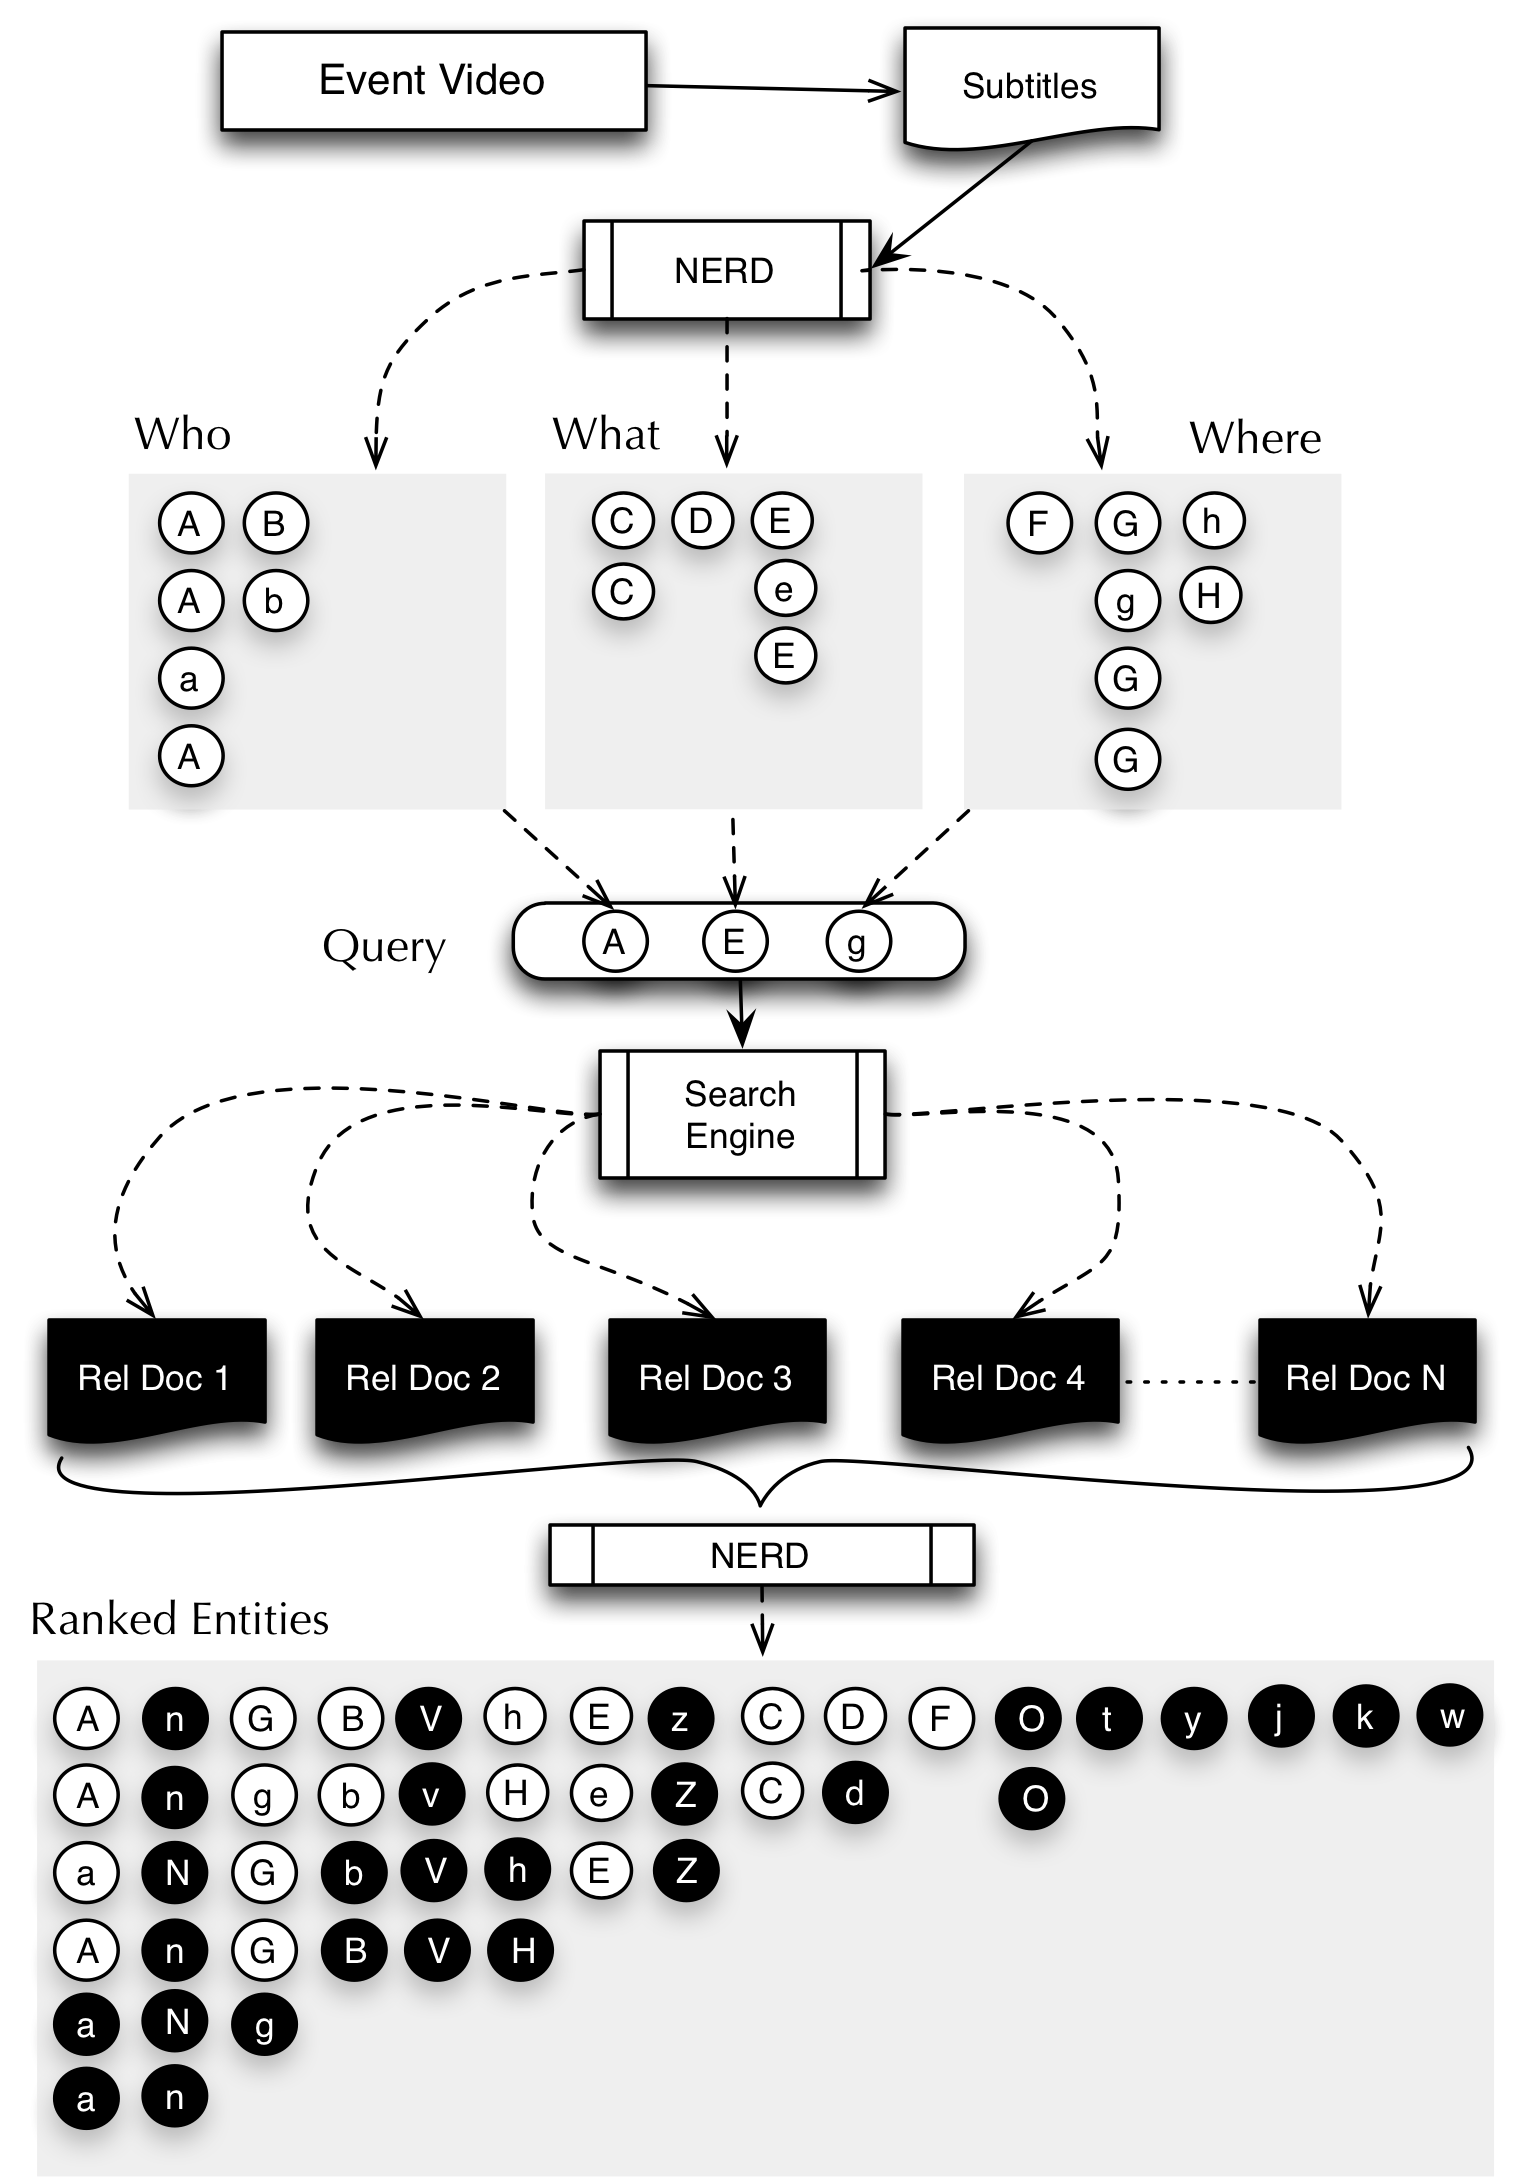
\includegraphics[width=0.4\textwidth]{figure/ExpansionDiagram}
\caption{Schema of Named Entity Expansion Algorithm.}
\label{fig:namedEntityExpansion}%\end{figure}
\end{figure}

\subsubsection{Query Generation}

The Five Ws is a popular concept in information gathering in journalistic reporting. It captures the main aspects of a story or incidence: who, when, what, where, and why~\cite{LiJia2007}. In this paper we try to represent the news item in terms of four of those five W's (who is involved in the event, where the event is taking place, what the event is about, and when has happened) in order to generate a query that retrieves documents having to with the same event.This is somewhat like what a normal user would tape in a Web search engine when looking for descriptive documents about the same news item.  

Firstly the original entities are mapped to the NERD Core ontology, which considers 10 main classes: Thing, Amount, Animal, Event, Function, Organization, Location, Person, Product and Time. From this ten categories we generalize into three: the Who from \url{http://nerd.eurecom.fr/ontology#Person} and \url{http://nerd.eurecom.fr/ontology#Organization}, the Where from \url{http://nerd.eurecom.fr/ontology#Location}, and the What from the rest of NERD types after discarding \url{http://nerd.eurecom.fr/ontology#Time} and \url{http://nerd.eurecom.fr/ontology#Amount} instances. The When or so-called temporal dimension does not need to be computed since it is provided by the video publisher as an inputs for this approach.

Having the three set of entities already generated, the next step consist in ranking them in relevance according to a weighted sum of two different dimensions: their frequency in the transcripts and their former relevance scores coming from the NE extractors. We have defined the function $\text{filterEntities}(S)$ for selecting the $n$ entities inside the set of entities $S$ whose relative relevance

\begin{equation}
R_{rel}\left ( e_{i}, S \right ) = R\left ( e_{i} \right ) / Avg \left ( R\left ( e_{i} \right )  \right )
\end{equation}

falls into the upper quarter of the interval 

\begin{equation}
\left [ max\left ( R_{rel}\left ( e_{i}, S \right )  \right ) -min\left (  R_{rel}\left ( e_{i}, S \right ) \right ) \right ]
\end{equation}

The final query is a pair

\begin{equation}
\text{Query}_{Event} =\left [ \text{textQuery}, t \right ]
\end{equation}

where \textit{textQuery} is the result of concatenating the labels of the most relevant entities in the sets Who, What, Where in that particular order

\begin{equation}
\begin{split}
\textit{textQuery} = \text{labels} ( \text{filterEntities}(Who) \\ + \text{filterEntities}(What) \\ + \text{filterEntities}(Where) )
\end{split}
\end{equation}

and $t$ the time period dimension. 
This query generation process is depicted in the upper part of . For future research in the query construction technique we plan to directly use the Web resources themselves and not only their labels. 

\subsubsection{Document Retrieval}

Once $\text{Query}_{Event}$ is built out of the original set of named entities it will be ready to be injected into a document search engine where additional descriptions about the news event can be found. In this situation, the kind of query generated in the previous step and the search engine chosen should be closely tied in order to maximize the quality of the obtained results. Of course the different behavior of different search engines make some alternatives more suitable than others for certain kinds of events. The way the resultant documents change along the different search engines for a particular kind of event is a research question that will not be studied in this paper.

For the work presented in this paper we have resorted to Google Search REST API service\footnote{Available at http://ajax.googleapis.com/ajax/services/search/web?v=1.0}  by launching a query with the text \textit{textQuery}. Due to quota restrictions imposed by Google, the maximum number of retrieved document is set to 30. However and according to the evaluation performed in Section~\ref{sec:evaluation} this number is already enough for significantly extending the initial set of entities directly spotted by NERD. 

In which concerns to the temporal dimension, we keep only the documents published inside the time period $t+t_{e}$. We increase the original event period in $t_{e}$ is because documents concerning a news event are not always published during the time the action is taking place but some hours or days after. The value of $t_{e}$ depends on many factors like the nature of the event itself (it is a quick appearance in the media, or a deep fact with more repercussion) or the kind of documents the search engine is indexing (from very deep and elaborated documents that need time to be published, to light post generated by users in just some minutes). Based on the simple assumption that that longer event will provoke longer buzzes, we approximated  $t_{e} = t$, meaning that we consider also document published duration of the event. 

In the middle part of Figure~\ref{fig:namedEntityExpansion} this process is shown. The query is inputted in the search engine for obtaining other documents that elaborate on the the same event mentioned in the original video.Those documents (colored in black in the figure) will be also further processed for increasing the size of the collection and getting extra insights about the the studied news item.

\subsubsection{Entity Clustering}

In this phase the extra documents previously retrieved are now preprocessed and analyzed in order to extend and rerank the original set of relevant entities and consequently get more insights about the studied event. First, since most of the retrieved resources are Web pages, HTML tags and other annotations are removed, keeping only the main textual information. This plain text is then analyzed by the NERD framework in order to extract the named entities present in them.

In order to calculate the frequency of a certain resource inside the entire corpora, we group the different appearances of the same instance and check their cardinality. This is not trivial since the same entity can appear under different text labels, contain typos in the field or have different disambiguation URL's pointing to the same resource. We therefore performed a centroid-based cluster operation over the instances of the entities. We considered the centroid of a cluster as the entity with the most frequent disambiguation URL that have also the most repeated labels. As distance metric for comparing pairs of entities we applied strict string similarity over the URL's, and in case of mismatch, Jaro-Winkler string distance~\cite{Winkler06overviewof} over the labels. The output of this phase is a list of clusters containing different instances of the same entity.

\subsubsection{Entity Ranking}

The final step of the expansion consists of ranking the different named entities obtained so far. To create this ordered list we assigned a score to every entity according to the following features: relative frequency of the entity in the transcripts of the event video; relative frequency of the entity over the extra document; and average relevance for the different instances according to the named entity extractors. The three dimensions are combined via a weighted sum where the relative frequency in the video subtitles has a bigger impact in the final score, followed by the relative frequency on the searched documents, and ending with a typically very variable average relevance from the extractors.

The final output of the entity expansion operation is a list of entities (normally filtered by a minimum number of appearances since the method brings a much higher number of candidate entities), together with their ranking score and the frequency in both the main video and in the collected extra documents.

\begin{equation}
\begin{split}
\text{EntityExpansion}\left (subtitles, timePeriod \right )= \\
\left ( \left \{ e_{i},  relScore_{i}, Freq\left ( subtitles, e_{i} \right ), Freq\left ( extraDocs, e_{i} \right ) \right \} \right )
\end{split}
\end{equation}

Entities with a higher $relScore_{i}$ in the final classification are more representative for the context of the original. Also there are other advantages in the final set of results:
\begin{itemize}
  \item The entities will be better ranked since the size of the sample is bigger. Entities appearing repeatedly in the extra documents will be promoted while those barely appearing in two or three documents will be at the end of the list.
  %TODO: documents?
  will have less relevance.
  \item Entities that originally have not been disambiguated can now have their corresponding URL if any of the similar instances appearing in the additional documents provide a link to a Web resource. The same occurs with labels containing errors or incomplete labels. 
  \item  Finally, some entities important in the context of the news item but not mentioned in the original transcripts, are now included in the list of relevant items since they have been often spotted over the collected documents. 
\end{itemize}


\subsection{Refining Event Context via DBPedia Knowledge}

Once the set of context relevant entities has been expanded, we will use knowledge of structured sources (e.g. DBpedia) for reinforcing the important entities and finding relevant predicates between them. 

\subsubsection{Generating DBpedia paths}
\label{sec:introduction}

Before we filter the relations between resources, the candidate resources to be included in relations are being pre-ranked. They are pre-ranked according to ``popularity'' and ``rarity'' essential components in the original PageRank algorithm \cite{page1999pagerank} and is used to sort candidate related nodes in the EiCE. The implementation of the EiCE takes the relations in to account by making use of the Jaccard coefficient to measure the dissimilarity and assign random walks based weight able to highly rank more rare resources, and guaranteeing that paths between resources prefer specific relations and not general ones \cite{moore2012novel}.

\begin{figure}[h!]
\centering
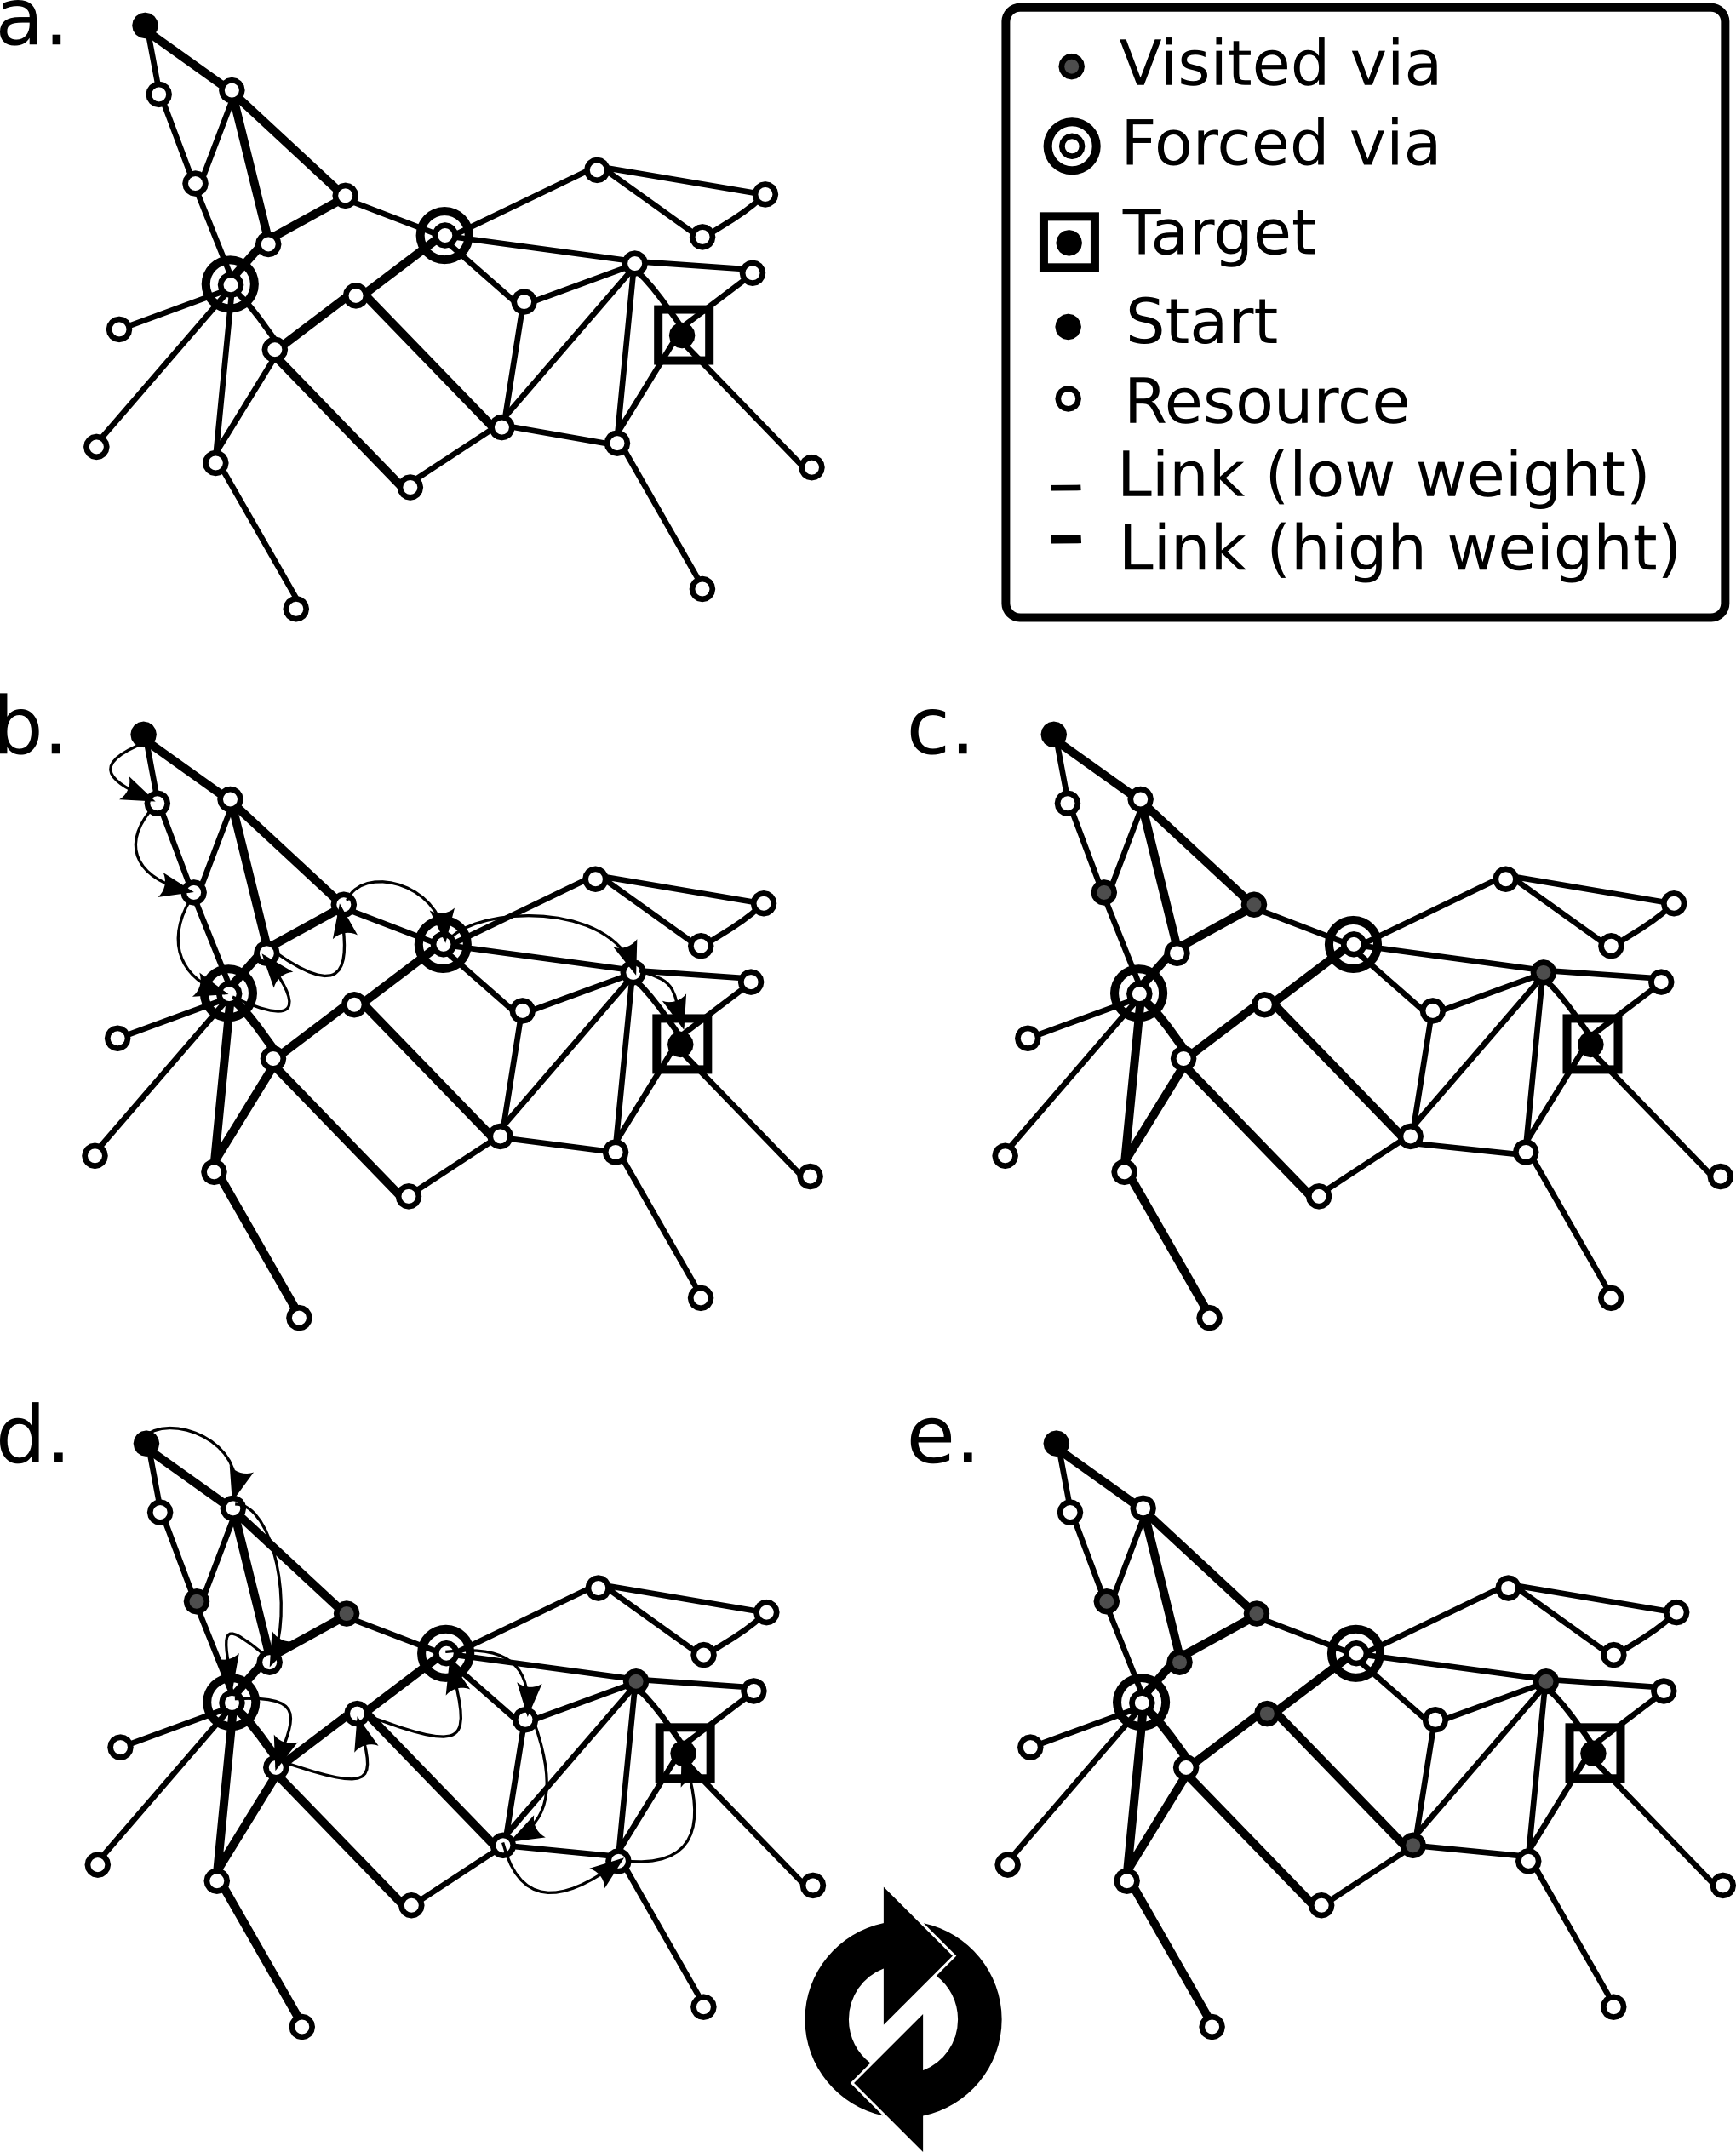
\includegraphics[width=0.4\textwidth]{graphmultipatternmatching.png}
\caption{Pattern matching with multiple results using an iterative pathfinding process.}
\label{fig:patternmatching}
\end{figure}

We pass on the main start resource, a target and via points. Figure~\ref{fig:patternmatching} shows the iterative process for generating DBpedia paths. An initial state is computed in step \ref{fig:patternmatching}a. There are low weights and high weights
%, for the example 1 and 2 respectively
. Based on the weights of the links te path through the vias is optimized, so a path with the lowest total weight will be selected first, until the vias are added to the exclude list. The path from start to end is forced through the given via points (\ref{fig:patternmatching}b). This leads to additional visited resource as via points (\ref{fig:patternmatching}c). They occur because to resolve each path, the route is being computed starting in the start resource, target and the via points. The resources where they converge to each other are considered as the new via points. These via points are included in the paths and therefore marked as visited. This is to make sure that in the next iteration paths will go around the visited via (\ref{fig:patternmatching}d). The next paths are being computed over and over (\ref{fig:patternmatching}e) until a threshold number of paths is found and the context is large enough or when it takes to long to compute the next path (out of range). The final set of optimized paths used to for the context expansion.

\subsubsection{Analyzing Context Relevant Paths}

In this step the DPpedia path finding technique implemented in ~\ref{sec:evaluation} will be applied over the set of entities obtained via entity expansion. However, this list is too big and broad. Before, we need to establish a division between the main entities (\textit{MainEntities}, entities with relative score higher than the average), and the additional entities (\textit{additionalEntities}, the rest of entities in $E_{Expansion}\left (subtitles, timePeriod \right )$). 

%in \url{demo.everythingisconnected.be/relations?uris=} 
Afterwards, we calculate paths between all the possible pairs inside the set\textit{MainEntities} following the REST methods exposed at \url{demo.everythingisconnected.be/relations?uris=}. Once all the possible paths have been retrieved, we perform various analysis for detecting which are the most frequent classes and predicates:
\begin{itemize}
  \item  We detect the most frequent nodes ($F_{nodes} = f_{max}(n_{i})$ in $Paths (mainEntities)$).
  \item  We detect the most frequent predicates ($F_{prop} = f_{max}(p_{i})$ in $Paths (mainEntities)$). The edges (DBpedia properties) will determine which are the most relevant properties inside the context of this news item.
  \item  We estimate the connectivity between nodes (Adjacency Matrix $M_{i,j}$ where the distance between two entities $e+{i}$ and $e+{j}$ is the average of the lengths of the paths that link those entities $m_{i,j} = \\ Avg (lenght(Paths(e_{i}, e_{j})))$)
\end{itemize}

The output of this process two different lists and a matrix: a re-expanded and re-ranked list of entities generated out of the expansion set, a list of the most important predicates involved in the paths between the aforementioned entities, and the adjacency matrix.

\begin{equation}
\begin{split}
\{ E_{Expansion}, F_{nodes}, F_{prop}, M_{i,j} \} \\
\end{split}
\end{equation}

\subsubsection{Reranking entities via Filtering}

Use the frequency measures obtained previously in order to rerank entities. Get intermediate items using the commonalities function for some top ranked items. Output final set of entities and adjacency matrix.

\begin{itemize}
  \item  Most frequent via nodes will reinforce entities already existing in $E_{Expansion}$.
  \item  Most frequent properties will feed Commonalities function over each entity in $mainEntities$
  \item  Most frequent entities in Commonalities will promote already existing in $E_{Expansion}$.
  \item  Most frequent via nodes will reinforce entities already existing in $E_{Expansion}$.
  \item  Most frequent via nodes will include new entities inside $E_{Expansion}$.
  \item  Final  $E_{Expansion}$.

The final output of the approach is the set of context entities rerank according to DBPedia insights, and the final matrix of Adjacency:
\begin{equation}
\begin{split}
\{ Entities_{Extension + DBpedia}, M_{i,j} \} \\
\end{split}
\end{equation}
\end{itemize}

%\url{http://demo.everythingisconnected.be/commonalities?between=http://dbpedia.org/resource/Lyon&and=http://dbpedia.org/resource/France&allowed=http://purl.org/dc/terms/spatial}

\section{Use Case: Snowden Assylum}

We have applied the explained approach over the video \url{http://www.bbc.co.uk/news/world-europe-23339199} from the BBC News Europe site. The main  story in this media content is the request of  asylum made by Edward Snowden to the Russian government. In an airport in Moscow, he publicy express  his desire to obtain political help while he can find a safe way to reach the Latin American countries offering to harbor him. The time period for which this particular part of the event is relevant goes from 2013/07/06 to 2013/07/17.

\subsection {Named Entity Extraction}

In a first step, Name Entity Extraction techniques are applied over the video transcript by using NERD. Below we show the different entities directly extracted with this procedure.

\resizebox{8.5cm}{!} {
\begin{tabular}{ c | c | c | c | c }
  \hline     
 Label & Relevance & Sentiment & Type & URI  \\ \hline  
Russia & 0.809216 & Mixed & Location & http://en.wikipedia.org/wiki/Russia \\
Edward Snowden & 0.717369 & Mixed & Person & http://en.wikipedia.org/wiki//Edward\_Snowden \\
South America & 0.56586 & Mixed & Location & http://en.wikipedia.org/wiki/South\_America \\
president Putin & 0.459811 & positive & Person & http://en.wikipedia.org/wiki/Vladimir\_Putin \\
president & 0.401138 & negative & JobTitle & http://en.wikipedia.org/wiki/President \\
Moscow & 0.352101 & Mixed & City & http://en.wikipedia.org/wiki/Moscow \\
CIA & 0.334887 & neutral & Organization & http://en.wikipedia.org/wiki/CIA \\
Bolivia & 0.324607 & neutral & Location & http://en.wikipedia.org/wiki/Bolivia \\
Obama & 0.321901 & negative & Person & http://en.wikipedia.org/wiki/Barack\_Obama \\
  \hline  
\end {tabular} 
  }

\subsection {Named Entity Expansion}

In the second step, the original set of entities is expanded and the items are rerank according to the procedure explained in 

%\url{curl -X POST --data-binary @snowden.txt "http://localhost:8006/api/rankedentities?startdate=2013-07-16&enddate=2013-08-15&limit=50" --header "Content-Type:text/xml" -v >> snowden_textrazor_50_130716_130815.json2}

\resizebox{9cm}{!} {
\begin{tabular}{ c | c | c | c | c | l }
  \hline     
  	Label & Relevance & $F_{video}$& $F_{Docu}$ & Type & URI \\ \hline                  
  	Russia & 0.571518 & 7 & 197 & Location & http://en.wikipedia.org/wiki/Russia \\ 
  	Edward\_Snowden & 0.485714 & 2 & 242 & Person & http://en.wikipedia.org/wiki/Edward\_Snowden \\
  	Asylum & 0.297630 & 4 & 84 & Thing & http://en.wikipedia.org/wiki/Right\_of\_asylum\\
  	United States & 0.261129 & 5 & 50 & Location & http://en.wikipedia.org/wiki/United\_States \\
  	Vladimir Putin & 0.2193704 & 1 & 99 & Person & http://en.wikipedia.org/wiki/Vladimir\_Putin \\
	Barack Obama & 0.1899647 & 1 & 89 & Person & http://en.wikipedia.org/wiki/Barack\_Obama \\
	MOSCOW & 0.173273 & 1 & 85 & Location & http://en.wikipedia.org/wiki/Moscow \\
	extradition & 0.1178356 & 2 & 14 & Thing & http://en.wikipedia.org/wiki/Extradition \\
	CIA & 0.116887 & 1 & 45 & Organization & http://en.wikipedia.org/wiki/CIA \\
	human-rights & 0.0767802 & 2 & 10 & Organization & http://en.wikipedia.org/wiki/Human\_rights \\
	Anatoly Kucherena & 0.0694218 & 0 & 42 & Person & -- \\
	Kremlin & 0.0662006 & 1 & 11 & Location & http://en.wikipedia.org/wiki/Kremlin \\
	Sheremetyevo & 0.0396691 & 0 & 24 & Location & http://en.wikipedia.org/wiki/Sheremetyevo\\

  \hline  
\end {tabular} 
  }

\subsection {Named Entity Expansion}

\section{Evaluation}
\label{sec:evaluation}

There result obtained by this approach will be evaluated against a set of entities provided by an expert. 
We plan to extend this evaluation to a larger corpora and include a more exhaustive evaluation in following publications in the same line.
This is the list of entities provided by the expert, together with some insights about the concept and its relations with the main topic in the video:

\begin{Verbatim}[fontsize=\tiny] 
Edward Joseph Snowden: (M)
o   Public figure. He is the "who" of the news.
o   The subject of the main sentence.
 
Political Asylum (M)
o   This is related to the �what� of the news. This is what he requested, the direct object.
 
CIA (M)
o   Background information on related to Snowden, the main subject of the news, "ex CIA employee".
o   An actor in the news in a wider sense, not this news in particular, but Snowden�s history.
 
Sheremetyevo Airport (NM)
o   Specific location of the news.
o   Mentioned as "the Moscow airport"
 
Anatoly Kucherena (NM)
o   Secondary actor and speaker in the video.
o   Information about an interview or person expressing his opinion.
 
Rusia (M)
o   The location, but also an actor, the indirect object of the main sentence "to whom".
 
US Department of State (NM)
o   Involved organization. Not mentioned but related to speaker.

\end{Verbatim}

Evaluating against traditional Named Entity Extraction: Precision \& Rec: there are 3 entities out of 7 spotted. 12 Entities in total
\begin{itemize}
  \item  The lawyer, behind the case, Anatoly Kucherena, is never mentioned in the 
  \item  The name of the airport. (There are two airport in Moscow, we don't know which one it is)
\end{itemize}

Evaluating against \textit{MainEntities} in $E_{Expansion}$: Precision \& Rec: there are 6 entities out of 7 spotted. 15 Entities in total
\begin{itemize}
  \item  Assylum, the main subject behind this news item, has been correctly detected
  \item  Anatoly Kucherena is the lawyer involved in the defense of Edward Snowden, has been correctly detected even there is no disambiguation URL.
  \item  The Name of the airport, Sheremetyevo, has been finally disambiguated. In the original transcript it was not specified in which of the two airports in Moscow Snowden was giving the press conference.
  \item  Other important entities like "human-rights" and "extradition" are now present, helping to complete the context of the new.
\end{itemize}

Evaluating against the final DBPedia $E_{Expansion + DBpedia}$: No differences for the  \textit{MainEntities} in which refers to Precision \& recall. However, there are improvements in which concerns:

\begin{itemize}
  \item  The ranking order inside  \textit{MainEntities} is now better. For example the entity "Sheremetyevo" is now scored higher, which is taking into account that it is the specific location where the action is taking place.
  \item  There are new entities that were not detected via entity expansion, like the prime Minister of Russia, Igor Shuvalov, that are also relevant inside the matter.
  \item  The matrix of Adjacency opens room for many other context studies, like topic entity clustering that could help to give extra insight about the studied event.

\section{Conclusions}
We presented a new approach for context-aware annotating news events. Our approach is designed to harvest highly precise contexts starting from named entities recognized in a TV fragment about the news event. Firstly we extracted named entities out of the corresponding subtitles and expanded those by collecting related documents to the news event. The entities obtained from the first pass typical are insufficient. Secondly we applied a second pass named entity extraction on these documents. We then ranked all the entities obtained at that stage and filter out those least occurring or identified as unimportant. Finally we refined the remaining entities by reinforcing them and finding important predicates between them. Ultimately this leaded to a re-ranking of the entities belonging to this news event.

Our preliminary results indicate that by exploring DBpedia paths in named entities occuring in news media.

\section{Future Work}
%Explain how we are going to use predicates.

%Mention refinements using TF/IDF weights.

%ACKNOWLEDGMENTS are optional
\section{Acknowledgments}
The research activities described in this paper were funded by Ghent University,
%iMinds (Interdisciplinary institute for Technology) a research institute founded by the Flemish Government,
the Institute for the Promotion of Innovation by Science and Technology in Flanders (IWT), the Fund for Scientific Research-Flanders (FWO-Flanders), and the European Union's 7th Framework Programme via the project LinkedTV (GA 287911).

%
% The following two commands are all you need in the
% initial runs of your .tex file to
% produce the bibliography for the citations in your paper.
\bibliographystyle{abbrv}
\bibliography{connectedEvents}  % sigproc.bib is the name of the Bibliography in this case
% You must have a proper ".bib" file
%  and remember to run:
% latex bibtex latex latex
% to resolve all references
%
% ACM needs 'a single self-contained file'!
%

\end{document}
